\documentclass[9pt]{beamer}

% --- Theme and Packages ---
\usetheme{Madrid}
\usecolortheme{beaver}
\usepackage{booktabs}
\usepackage{listings}
\usepackage{xcolor}
\usepackage{tikz}
\usetikzlibrary{positioning}
\usepackage{amsmath}
\usepackage{ragged2e}
\usepackage{url}

% --- Custom Definitions ---
\definecolor{googleblue}{RGB}{66, 133, 244}
\definecolor{googlered}{RGB}{219, 68, 55}
\definecolor{googleyellow}{RGB}{244, 180, 0}
\definecolor{googlegreen}{RGB}{15, 157, 88}
\definecolor{darkgray}{gray}{0.3}

\setbeamercolor{block title}{bg=googleblue,fg=white}
\setbeamercolor{alerted text}{fg=googlered}
\setbeamercolor{structure}{fg=darkgray}

% --- Code Style ---
\lstset{
    language=Python,
    basicstyle=\ttfamily\footnotesize,
    keywordstyle=\color{googleblue}\bfseries,
    stringstyle=\color{googlegreen},
    commentstyle=\color{gray}\itshape,
    showstringspaces=false,
    frame=single,
    rulecolor=\color{black!30},
    breaklines=true,
    breakatwhitespace=true,
    postbreak=\mbox{\textcolor{gray}{$\hookrightarrow$}\space},
    tabsize=2,
    columns=fullflexible
}

% --- Title ---
\title[AI Travel Architect]{AI Travel Architect: Project Deep Dive}
\subtitle{A Stateful Multi-Agent Travel Planning System}
\author{Martina Speciale}
\institute{Travel-Agent-AI}
\date{\today}

\setbeamertemplate{navigation symbols}{}

\begin{document}

\begin{frame}
    \titlepage
\end{frame}

\begin{frame}{Project Goal and Scope}
\begin{block}{Objective}
Build an autonomous travel planner that turns a user request
(destination, dates, budget, interests, companion) into a realistic itinerary
with verifiable places and actionable outputs.
\end{block}

\textbf{Core requirements}
\begin{itemize}
    \item Persistent state across reasoning steps (not a single prompt call).
    \item Grounding on real-world data (places and flight options).
    \item Self-correction loop when the plan is inconsistent.
    \item Human-in-the-Loop (HITL) when confidence is low.
    \item Deliverables in multiple formats: terminal, HTML, and DOCX.
\end{itemize}
\end{frame}

\begin{frame}{Architecture at a Glance}
\begin{columns}[t]
\column{0.52\textwidth}
\textbf{Implementation stack}
\begin{itemize}
    \item Orchestration: \textbf{LangGraph}
    \item LLM policy: \textbf{Groq} (+ optional fallback)
    \item Place grounding: \textbf{Google Maps Places API}
    \item Flight grounding: \textbf{SerpApi (Google Flights)}
    \item Route normalization: \textbf{local city\(\to\)IATA seed CSV}
    \item Artifacts: \textbf{HTML + DOCX publisher}
\end{itemize}

\column{0.48\textwidth}
\textbf{Code map}
\begin{itemize}
    \item State schema: \texttt{app/core/state.py}
    \item Node logic: \texttt{app/engine/nodes.py}
    \item Graph wiring: \texttt{app/graph.py}
    \item Tools: \texttt{app/tools/*.py}
    \item Observability: \texttt{app/core/logger.py}
\end{itemize}
\end{columns}
\end{frame}

\begin{frame}{Execution Graph (LangGraph Flow)}
\centering
\vspace{-0.15cm}
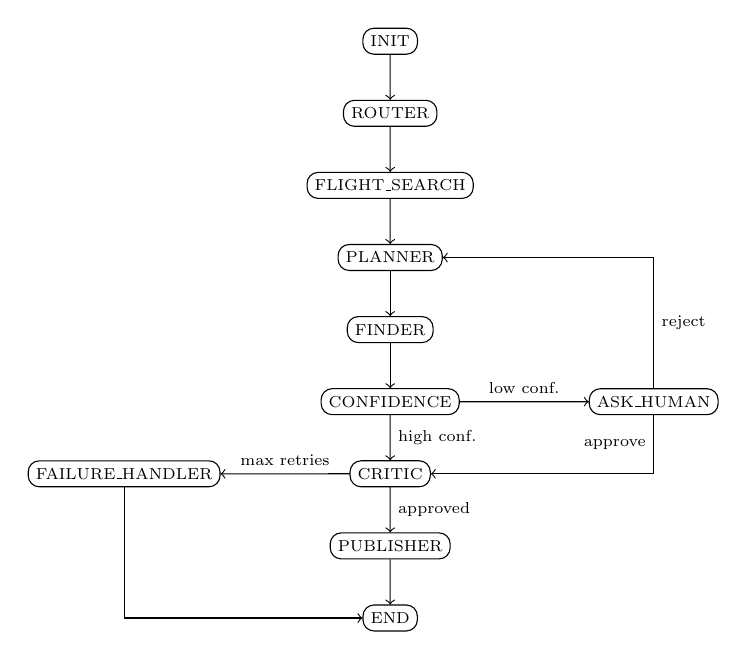
\begin{tikzpicture}[
    node distance=0.70cm,
    every node/.style={font=\scriptsize, transform shape},
    scale=0.82
]
    \node (init) [draw, rounded corners] {INIT};
    \node (router) [draw, rounded corners, below=of init] {ROUTER};
    \node (flight) [draw, rounded corners, below=of router] {FLIGHT\_SEARCH};
    \node (planner) [draw, rounded corners, below=of flight] {PLANNER};
    \node (finder) [draw, rounded corners, below=of planner] {FINDER};
    \node (conf) [draw, rounded corners, below=of finder] {CONFIDENCE};
    \node (critic) [draw, rounded corners, below=of conf] {CRITIC};
    \node (pub) [draw, rounded corners, below=of critic] {PUBLISHER};
    \node (endn) [draw, rounded corners, below=of pub] {END};

    \node (hitl) [draw, rounded corners, right=2.0cm of conf] {ASK\_HUMAN};
    \node (fail) [draw, rounded corners, left=2.0cm of critic] {FAILURE\_HANDLER};

    \draw[->] (init) -- (router);
    \draw[->] (router) -- (flight);
    \draw[->] (flight) -- (planner);
    \draw[->] (planner) -- (finder);
    \draw[->] (finder) -- (conf);
    \draw[->] (conf) -- node[right] {high conf.} (critic);
    \draw[->] (critic) -- node[right] {approved} (pub);
    \draw[->] (pub) -- (endn);

    \draw[->] (conf) -- node[above] {low conf.} (hitl);
    \draw[->] (hitl) |- node[pos=0.25,right] {reject} (planner);
    \draw[->] (hitl) |- node[pos=0.25,left] {approve} (critic);
    \draw[->] (critic) -- node[above] {max retries} (fail);
    \draw[->] (fail) |- (endn);
\end{tikzpicture}
\end{frame}

\begin{frame}{Flow Commentary: What Each Node Does}
\small
\begin{enumerate}
    \item \textbf{INIT} --- collects user constraints (destination, dates, budget, companion) and initializes shared state.
    \item \textbf{ROUTER} --- infers travel style and normalizes intent for downstream planning.
    \item \textbf{FLIGHT\_SEARCH} --- resolves city$\rightarrow$IATA, proposes best outbound/return flight, asks user confirmation.
    \item \textbf{PLANNER} --- generates a day-by-day draft itinerary coherent with style, dates, and budget signal.
    \item \textbf{FINDER} --- grounds each proposed place via Google Maps (address/rating), marking verified vs non-verified.
    \item \textbf{CONFIDENCE} --- computes reliability score from verified-place ratio; if low ($<0.7$), triggers HITL.
    \item \textbf{ASK\_HUMAN} --- interruption node: user can approve continuation or reject and force re-planning.
    \item \textbf{CRITIC} --- validates feasibility and consistency (logistics + budget plausibility); approves or sends feedback.
    \item \textbf{PUBLISHER} --- generates final artifacts (terminal, HTML, DOCX) once approved.
    \item \textbf{FAILURE\_HANDLER} --- safe exit after max retries, with explicit failure reason.
\end{enumerate}
\end{frame}

\begin{frame}{Shared Memory: TravelAgentState}
\textbf{Persistent graph state (TypedDict)}
\begin{itemize}
    \item Input: \texttt{destination}, \texttt{interests}, \texttt{budget}, \texttt{companion}, \texttt{origin}, \texttt{depart\_date}, \texttt{return\_date}
    \item \texttt{days}: auto-computed from dates when possible, otherwise requested explicitly
    \item Planning output: \texttt{travel\_style}, \texttt{itinerary}
    \item Flight output: \texttt{flight\_options}, \texttt{flight\_summary}
    \item Control fields: \texttt{confidence\_score}, \texttt{critic\_feedback}, \texttt{retry\_count}, \texttt{is\_approved}
    \item Context fields: \texttt{banned\_places}
\end{itemize}

\begin{block}{Why this matters}
The state is the memory backbone of the system: each node reads/writes a shared
object, enabling trajectory-level reasoning and deterministic routing decisions.
\end{block}
\end{frame}

\begin{frame}{Node Responsibilities}
\begin{columns}[t]
\column{0.5\textwidth}
\textbf{Decision nodes}
\begin{itemize}
    \item \textbf{Router}: validates and normalizes user request.
    \item \textbf{Flight\_Search}: resolves route and proposes outbound/return option.
    \item \textbf{Planner}: generates day-by-day itinerary draft.
    \item \textbf{Finder}: enriches draft with real places and ratings.
    \item \textbf{Critic}: checks feasibility (timing, distances, budget).
\end{itemize}

\column{0.5\textwidth}
\textbf{Control nodes}
\begin{itemize}
    \item \textbf{Confidence}: estimates reliability after grounding.
    \item \textbf{Ask\_Human}: interruption point for approval/edits.
    \item \textbf{Publisher}: renders final itinerary to artifacts.
    \item \textbf{Failure\_Handler}: safe termination after retries.
\end{itemize}
\end{columns}
\end{frame}

\begin{frame}{Grounding and Tooling Strategy}
\begin{block}{Real-world grounding pipeline}
Plan text is converted into concrete places, then validated with external data.
\end{block}

\begin{itemize}
    \item \textbf{Google Maps Tool}: resolves locations, addresses, ratings.
    \item \textbf{SerpApi Flights Tool}: retrieves structured flight options (one-way/return).
    \item \textbf{IATA seed resolver}: maps city names (IT/EN variants) to airport codes.
    \item \textbf{Robust tool interface}: tools return usable error strings, not crashes.
    \item \textbf{Confidence signal}: based on verified vs non-verified places ratio.
\end{itemize}

\begin{alertblock}{Failure mode addressed}
Without grounding, LLMs can output plausible but non-existent places.
Tool-verified retrieval reduces hallucinations and improves itinerary trust.
\end{alertblock}
\end{frame}

\begin{frame}{Self-Correction and HITL}
\textbf{Quality loop}
\begin{enumerate}
    \item Planner proposes itinerary.
    \item Critic checks consistency and constraints.
    \item If rejected, planner retries with critic feedback.
    \item After max retries, graph exits via failure handler.
\end{enumerate}

\textbf{Human-in-the-Loop trigger}
\begin{itemize}
    \item If \texttt{confidence\_score < 0.7},
    execution pauses for human confirmation.
    \item User can approve (continue) or reject (re-plan).
\end{itemize}
\end{frame}

\begin{frame}{Observability and Outputs}
\begin{columns}[t]
\column{0.52\textwidth}
\textbf{Observability}
\begin{itemize}
    \item Structured, color-coded logs for node actions.
    \item Trace of \textit{thought vs action} transitions.
    \item Easier debugging of trajectory failures.
\end{itemize}

\column{0.48\textwidth}
\textbf{Delivered artifacts}
\begin{itemize}
    \item Terminal itinerary summary.
    \item \textbf{HTML report} with map-oriented layout.
    \item \textbf{DOCX report} for editable handoff.
\end{itemize}
\end{columns}

\vspace{0.2cm}
\begin{block}{Engineering payoff}
The output is not only text generation: it is a reproducible, inspectable,
and user-ready travel artifact.
\end{block}
\end{frame}

\begin{frame}{Limitations and Next Iteration}
\textbf{Current limitations}
\begin{itemize}
    \item API dependency (availability, quotas, response drift).
    \item Confidence score is heuristic, not fully calibrated.
    \item Critic quality depends on prompt quality and itinerary structure.
\end{itemize}

\textbf{Planned improvements}
\begin{itemize}
    \item Automatic evaluation set (golden prompts + regression checks).
    \item Better international city/airport coverage in the local seed.
    \item Stronger date parsing and calendar constraints.
    \item Optional cost signals from richer place metadata.
    \item Native timeline map in final HTML output.
\end{itemize}
\end{frame}

\begin{frame}{Takeaways}
\begin{block}{What this project demonstrates}
A production-oriented agent is a system, not a single model call:
\textbf{policy + controller + state + tools + evaluation loop}.
\end{block}

\begin{itemize}
    \item Stateful orchestration enables robust multi-step reasoning.
    \item External tools provide grounding and reduce hallucinations.
    \item Critic/HITL loops improve reliability under uncertainty.
    \item Observability turns debugging into an engineering workflow.
\end{itemize}
\end{frame}

\end{document}
